%%%%%%%%%%%%%%%%%%%%%%%%%%%%%%%%%%%%%%%%%%%%%%%%%%%%%%%%%%%%%%%%%%%%%%%%%%%
%%%                         O MODELO                                    %%%
%%%%%%%%%%%%%%%%%%%%%%%%%%%%%%%%%%%%%%%%%%%%%%%%%%%%%%%%%%%%%%%%%%%%%%%%%%%

\chapter{Descrição do Projeto}

% objetivos, ponto de partida, produtos e resultados esperados, tecnologias a serem usadas.
% + estrutura da solução nas fases de treinamento e aplicação

% ### METODOLOGIA ###

% ### Falar das seguintes ferramentas:
%   - DSR ok
%   - Trello
%   - Github

A seguir, serão apresentadas a metodologia e os softwares utilizados neste estudo, bem como as etapas detalhadas de sua implementação.

% Metodologia
\section{Metodologia}~\label{sec:metodologia}
Um ponto importante para a obtenção dos objetivos deste trabalho está relacionada a definição da metodologia que servirá como alicerce. Com a proposta de desenvolver e validar um método de análise da evolução molecular de vírus com base no uso de códons, a metodologia escolhida para isso é o \gls{dsr}. Essa metodologia, proporciona um framework teórico e prático para a criação de artefatos inovadores, como métodos, modelos ou frameworks, visando resolver problemas específicos~\cite{peffers_dsr_2007}. Neste projeto, a ferramenta de análise de genes virais baseada em códons é o artefato que será desenvolvido e avaliado. Além disso, o \gls{dsr} enfatiza a validação e a avaliação da utilidade e eficácia do artefato em relação aos seus objetivos práticos. No caso deste projeto, a validação será realizada através da comparação dos resultados obtidos com a ferramenta proposta em relação às técnicas clássicas filogenéticas, que são amplamente utilizadas para a análise de genes virais. Essa comparação permitirá avaliar a eficácia e o valor agregado da abordagem baseada em códons.

Para a obtenção de sucesso ao utilizar o \gls{dsr} os seguintes passos serão seguidos:
\begin{enumerate}
  \item \textbf{Identificação do problema e definição dos objetivos:} Nesta fase, o problema a ser resolvido é identificado e compreendido em detalhes. No contexto deste projeto, isso envolveria a compreensão das limitações das abordagens existentes para a classificação de genes virais.
  \item \textbf{Concepção e planejamento:} Aqui, são definidos os objetivos do artefato a ser criado, suas características e funcionalidades. No projeto em questão, isso envolveria a definição da funcionalidade da ferramenta de análise de genes virais com base em códons.
  \item \textbf{Desenvolvimento dos artefatos:} Nesta fase, o artefato é desenvolvido. Para o projeto, isso incluiria a criação dos scripts de download, processamento, tradução de sequências, algoritmos de agrupamento e outras partes da ferramenta.
  \item \textbf{Avaliação do artefato:} O artefato é testado e avaliado quanto à sua eficácia na resolução do problema. Isso pode incluir testes de desempenho, experimentos e comparações com métodos existentes.
  \item \textbf{Apresentar contribuições científicas:} Os resultados e contribuições do artefato são comunicados, geralmente por meio de artigos científicos e relatórios técnicos.
  \item \textbf{Iteração:} O processo é iterado conforme necessário. À medida que novos problemas ou insights surgem, o artefato é aprimorado.
\end{enumerate}

Sendo assim, como apresentado na figura\ref{fig:processoDSR}, os passos citados anteriormente são realizados em uma iteração constante, até a obtenção do objetivo final.

\begin{figure}[htb]
  \centering
  \caption{Processo iterativo da metodologia \gls{dsr}.}
  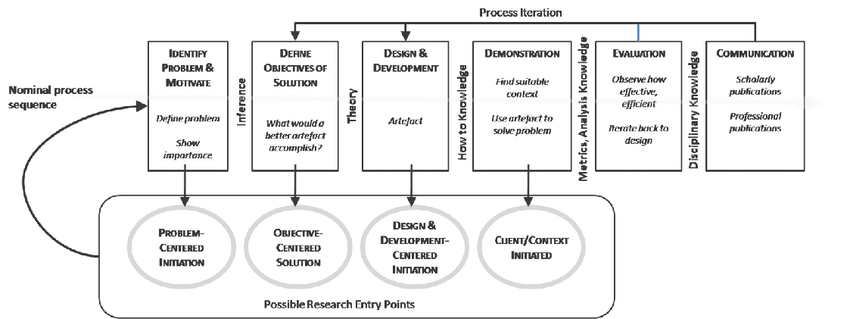
\includegraphics[scale=0.6]{figuras/Design-Science-Research.png}
  \fonte{O Autor}~\label{fig:processoDSR}
\end{figure}

% FAZER
% Para auxiliar no processo de gerenciamento e desenvolvimento dos artefatos, foram utilizadas outras duas ferramentas, trello e github...
% Escrever sobre as ferramentas
Também será utilizada análises quantitativas, ou seja, medidas estatísticas para mensurar e comparar os resultados obtidos.\\
A pesquisa quantitativa só tem sentido quando há um problema muito bem definido e há informação e teoria a respeito do objeto de conhecimento, entendido aqui como o foco da pesquisa e/ou aquilo que se quer estudar. Esclarecendo mais, só se faz pesquisa de natureza quantitativa quando se conhece as qualidades e se tem controle do que se vai pesquisar~\cite{da_silva_pesquisa_2014}.

\section{Materiais e Métodos}
Nesta sessão, será apresentada as ferramentas utilizadas para a construção e desenvolvimento de todo o trabalho.

O Python é uma linguagem de programação de alto nível, interpretada, iterativa e de código aberto. Foi criada por Guido van Rossum e lançada em 1991. A linguagem é conhecida por ter uma sintaxe simples, tornando-a popular para o desenvolvimento de software, automação, análise de dados, aprendizado de máquina entre outras aplicações. A mesma apresenta suporte a vários paradigmas de programação, como a orientada a objetos, imperativa, procedural e funcional. Além disso, o Python é portátil, podendo ser executado em diversos sistemas operacionais como Linux, Mac e Windows~\cite{python-reference}.

Para a construção dos pipelines do projeto, utilizamos Python em conjunto com o Jupyter Notebook. O Jupyter Notebook é uma aplicação de código aberto que permite criar documentos interativos que integram código, texto narrativo e visualizações. É uma ferramenta amplamente adotada por cientistas de dados, pesquisadores e desenvolvedores para explorar dados, prototipar código, documentar projetos e facilitar a colaboração. Além disso, o Jupyter Notebook oferece suporte a diversas linguagens de programação, incluindo Python~\cite{jupyter-notebook}.

O python possui uma gama de bibliotecas que facilitam a implementação de soluções complexas. A seguir serão apresentadas a bibliotecas utilizadas:

\begin{itemize}
  \item \textbf{Biopython}: Coleção de bibliotecas e ferramentas em Python, disponíveis gratuitamente para biologia molecular computacional. Ele fornece uma ampla gama de funcionalidades, desde a leitura e análise de arquivos de sequência biológica até a execução de algoritmos sofisticados de bioinformática. Desenvolvida e mantida pelo Projeto Biopython, que é uma associação internacional de desenvolvedores de ferramentas python~\cite{biopython}.
  \item \textbf{Selenium}: Biblioteca de código aberto que fornece uma interface programática para automatizar interações com navegadores da web. É amplamente utilizado por desenvolvedores e testadores de software para realizar testes automatizados, raspagem de dados na web e outras tarefas que envolvem interações com páginas da web. O Selenium para Python permite a automação de ações como clicar em botões, preencher formulários, navegar em sites e extrair informações da web, tornando-o uma ferramenta valiosa para desenvolvimento e automação de tarefas na web~\cite{selenium-python}.
\end{itemize}

% Lista de Tecnologias/Ferramentas utilizadas:
% Python 3 ok
% Selenium ok
% Biopython ok
% Shell (verificar necessidade)
% Jupyter Notebook ok
% Minimap2
% GoFasta
% virtualEnv
% AGUA (verificar e apresentar os sub-softwares utilizados, ex.: CLOPE)
% BV_BRC - O \gls{bvbrc}, é um centro de recursos de bioinformática dedicado ao estudo e análise de bactérias e vírus. O site também disponibiliza uma uma coleção abrangente de banco de dados, incluindo sequências genômicas, anotações funcionais, informações de expressão gênica e estruturas tridimensionais. O acesso aos bancos de dados é dado por meio de uma interface amigável, onde é possível realizar pesquisas avançadas.

\section{Plano de Implementação}
Durante o desenvolvimento do projeto foi necessário dividir o projeto em fases com base nas atividades que deveriam ser realizadas de forma a atender todos os passos descritos na seção~\ref{sec:metodologia}. As principais fases identificadas foram: Montagem e preparação do dataset a ser utilizado pelo modelo; Desenvolvimento completo do modelo, com todos as definições, implementações, testes e correções necessárias; e a análise comparativa que será realizada com um outro método existente e já tradicional. Esses pontos são apresentados de forma minuciosa a seguir.

\subsection{Montagem e Preparação do Dataset}
% Verificar como descrever os dois conjuntos de pipelines montados. Pip 01 (Descartado) - Pip 02 (Atual)
% FAZER
% Adicionar nota de rodapé com o link do repositório no Github
% Adicionar que o máximo de sequências baixadas por tipo foi de 10000 (dez mil). Limite máximo de sequências por vez aplicado pela própria plataforma. Sendo selecionadas as primeiras 10k
Para realizar o treinamento do modelo a ser construído, eram necessárias sequências únicas e alinhadas do gene Spike. Em vista disso, é importante salientar que o site \gls{bvbrc} disponibiliza sequências genômicas, e sendo assim, foi preciso construir um pipeline para, após o download das sequências, transformar as mesmas para a criação de um dataset com as sequências que atendessem os requisitos esperados.

Inicialmente, foi realizada uma analise do \gls{bvbrc}, para entende a sua estrutura e verificar também se era possível realizar o download de todas as sequências queridas de forma manual. Foi verificado que o site possuía uma área de seleção de filtros, e foi definido que só seriam selecionadas sequências completas no campo \textit{Genome Status} e no campo \textit{Lineage}, onde é possível filtrar as sequências pelo seu tipo \textit{Pango} e também verificar a quantidade, só os que tivessem mais de 50 sequências do mesmo tipo.

Após a análise, foi constatado que realizar o download manualmente era infactível, e que seria preciso automatizar esse processo de iteração com a página, como vistos na Figura~\ref{fig:pipelineBvbrc}. Isto posto, foi realizado uma sequência de passos conhecidos como \textit{Web Scrapping} utilizado o Python juntamente com o Selenium, apresentados em seguida:

\begin{figure}[htb]
  \centering
  \caption{Pipeline de Download das Sequências Genômicas.}
  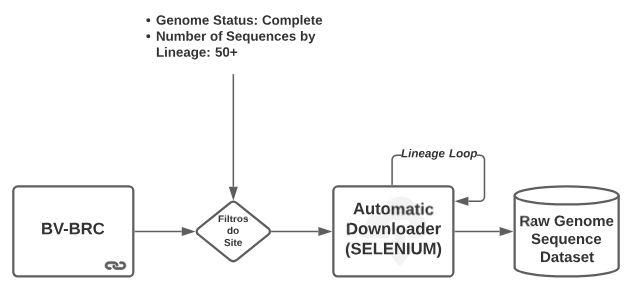
\includegraphics[scale=0.6]{figuras/pipelines/bvbrc.png}
  \fonte{O Autor}~\label{fig:pipelineBvbrc}
\end{figure}

\begin{enumerate}
  \item Criar uma lista com todos as linhagens disponíveis e a quantidade de sequências de cada.
  \item Desenvolver script Python para remover as linhagens com menos de 50 sequências da lista.
  \item Desenvolver script Python para gerar uma url personalizada do \gls{bvbrc}, já com os filtros, para cada linhagem.
  \item Desenvolver script Python juntamente com o Selenium para abrir as urls de forma automática e realizar o download das sequências.
\end{enumerate}

Ao final do processo de montagem do dataset, realizado no dia 02 junho de 2023, com sequências genômicas completas, foi gerado um diretório raiz (dataset), e dentro deste, um diretório para cada linhagem (\textit{Lineage} L¹, \textit{Lineage} L², \dots, \textit{Lineage} $L^{n}$), contendo um arquivo nomeado \textnormal{BVBRC\_genome\_sequence.fasta}, como apresentado na figura~\ref{fig:datasetGenomas}.

\begin{figure}[htb]
  \centering
  \caption{Dataset de sequências genômicas.}
  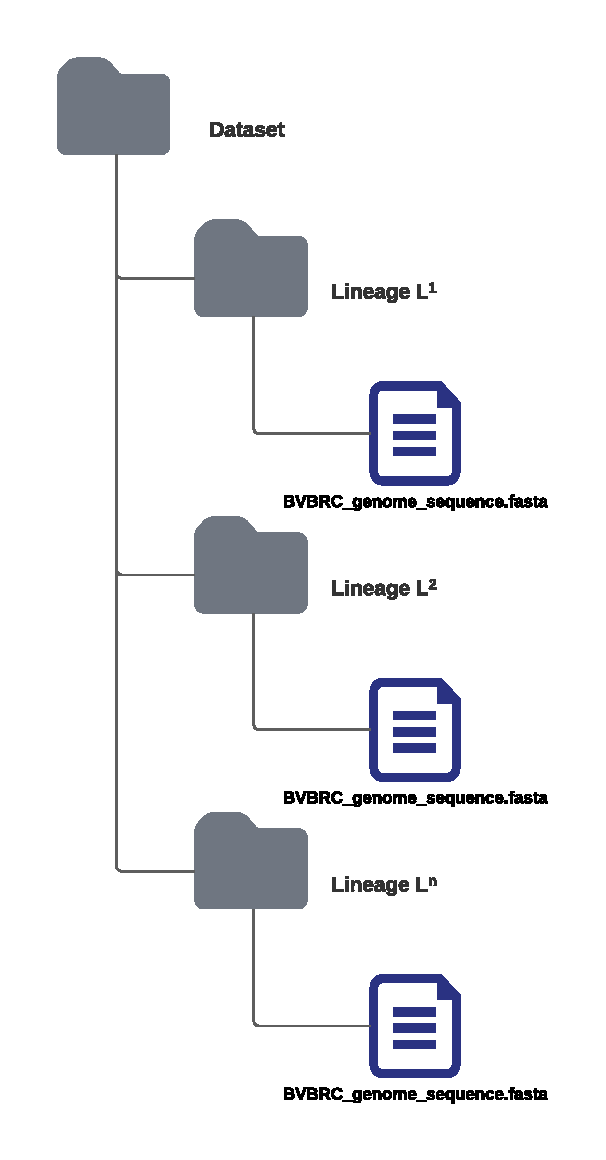
\includegraphics[scale=0.5]{figuras/dataset_principal.pdf}
  \fonte{O Autor}~\label{fig:datasetGenomas}
\end{figure}

Ao finalizar o processo de download, o \textit{dataset} completo ficou com as seguintes informações apresentadas na tabela~\ref{tab:datasetGenomas}.

%%tabela
\begin{table}[htb]
  \caption{Informações do dataset de sequências genômicas.}
  \begin{center}
    \begin{tabular}{c|c}
      \hline
      Campo                              & Valor     \\
      \hline
      Quantidade de Linhagens            & 1086      \\
      Quantidade de Sequências Genômicas & 1.494.650 \\
      Tamanho em \gls{gigabyte}          & 47.5      \\
      \hline
    \end{tabular}
  \end{center}
  \fonte{Criada pelo autor.}\label{tab:datasetGenomas}
\end{table}

A seguir, era necessário construir um dataset de sequências do gene Spike a partir do existente. Para isso, com o objetivo de diminuir o tempo de execução dos pipelines durante o desenvolvimento, foi construído também, um dataset de testes, apresentado na tabela~\ref{tab:datasetGenomasTeste}, que serviria como base para execução das atividades, e após as verificações, seria realizado o processo com o dataset completo. No dataset de testes, foram escolhidas 5 (cinco) linhagens que são amplamente conhecidas (gamma, delta, alpha, beta e omicron), o que tornaria mais preciso o processo de validação futuramente.

\begin{table}[htb]
  \caption{Informações do dataset de teste de sequências genômicas.}
  \begin{center}
    \begin{tabular}{c|c|c|c}
      \hline
      Pango     & \gls{who} & Quantidade de Sequências & Tamanho em \gls{megabyte} \\
      \hline
      B.1.1.7   & Alpha     & 9982                     & 307                       \\
      B.1.1.529 & Omicron   & 3694                     & 112.7                     \\
      B.1.351   & Beta      & 5256                     & 160.6                     \\
      B.1.617.2 & Delta     & 9996                     & 305.3                     \\
      P.1       & Gamma     & 10000                    & 305.9                     \\
      \hline
      Total     &           & 38928                    & 1191,5                    \\
      \hline
    \end{tabular}
  \end{center}
  \fonte{Criada pelo autor.}\label{tab:datasetGenomasTeste}
\end{table}

Depois, foi verificado a existência de sequências genômicas idênticas, melhor dizendo, sequências com exatamente a mesma quantidade e ordem dos nucleotídeos. Por isso, foi necessário desenvolver um pipeline que filtrasse as sequências repetidas, e mantivesse apenas uma, como exibido na figura~\ref{fig:pipelineGenomicasDuplicadas}, gerando assim um novo dataset de sequências genômicas únicas.

\begin{figure}[htb]
  \centering
  \caption{Pipeline de Filtragem de Sequências Genômicas Duplicadas.}
  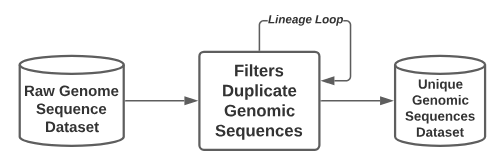
\includegraphics[scale=0.6]{figuras/pipelines/seqs_genomicas_duplicadas.png}
  \fonte{O Autor}~\label{fig:pipelineGenomicasDuplicadas}
\end{figure}

Com o dataset de sequências únicas montado, foi decidido os passos a seguir, que seriam executados com o papel de atingir o objetivo de obter o dataset de sequências gênicas únicas e alinhadas. Primeiro, como visto na figura~\ref{fig:pipelinesDescontinuados}, foi realizado o processo de extração do gene Spike, utilizando uma sequência de referência do gene obtida do dataset da \gls{ncbi}\footnote{Url para download: \url{https://www.ncbi.nlm.nih.gov/nuccore/NC_045512.2?report=genbank&from=21563&to=25384}}, juntamente com o software Blast, para encontrar e extrair o gene Spike de cada uma das sequências genômicas de todo o dataset. Após isso, com o dataset de sequências genicas já montado, era necessário realizar o processo de alinhamento das sequências. Foram verificada duas formas de realizar esse procedimento utilizando o software Clustalo Omega, uma passando uma sequência por vez (\textit{sequence by sequence}) com a sequência do Spike de referência e outra passando todas as sequências com a referência (\textit{multiple sequence}). Mesmo com o dataset de teste, que possuía um tamanho e quantidade de sequências muito inferior ao principal, o processo de alinhamento apresentou uma demora excessiva (até 2 dias) para finalizar. Em decorrência disso, o processo foi descontinuado, e um novo foi repensado e reconstruído e será apresentado a seguir.

\begin{figure}[htb]
  \centering
  \caption{Pipelines descontinuado.}
  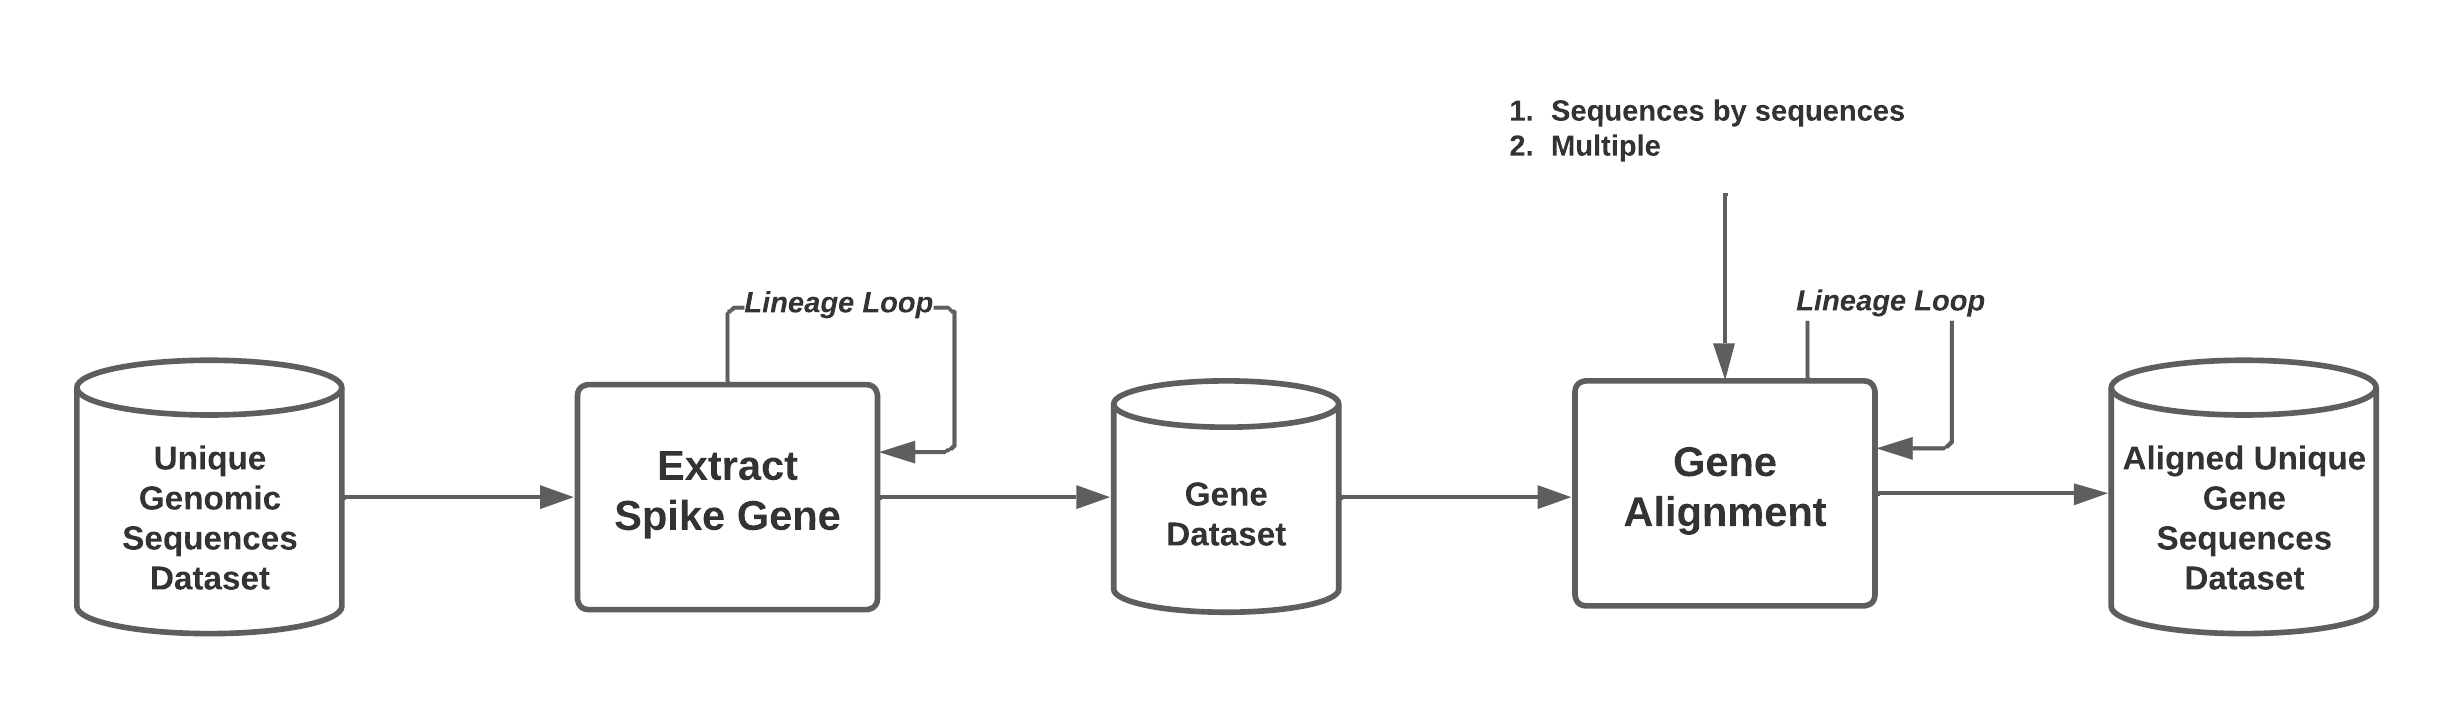
\includegraphics[scale=0.45]{figuras/pipelines/pipelines_descontinuado.png}
  \fonte{O Autor}~\label{fig:pipelinesDescontinuados}
\end{figure}

% FAZER
% Como escrever essa parte: Após análise; Após orientação do coorientador...
% Reescrever a lista abaixo de forma descritiva
% Substituir onde estiver citando 'modelo desenvolvido' pelo nome AGUA
Após um processo de análise, o desenvolvimento continuou a partir das sequências genômicas únicas, foi feito seguindo os quatro (4) passos apresentados a seguir:

\begin{enumerate}
  \item \textbf{Alinhamento das sequências genômicas:} A primeira etapa, como apresentado na figura~\ref{fig:alinhamentoGenomas}, consistiu em alinhar as sequências genômicas únicas já disponíveis, utilizando a ferramenta de alinhamento Minimap2. O Minimap2 é uma ferramenta eficiente para mapear sequências genômicas em um genoma de referência. Esse processo permitiu a identificação de regiões específicas relacionadas ao gene spike nas sequências genômicas.
        \begin{figure}[htb]
          \centering
          \caption{Pipeline de Alinhamento de Sequências Genômicas Duplicadas.}
          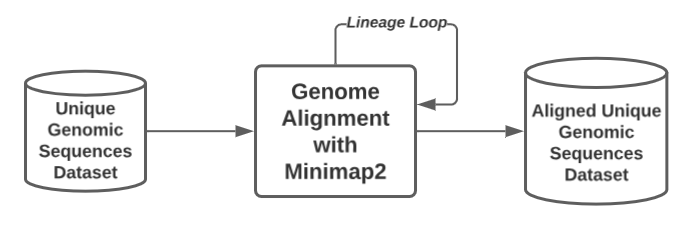
\includegraphics[scale=0.45]{figuras/pipelines/alinhamento_genoma.png}
          \fonte{O Autor}~\label{fig:alinhamentoGenomas}
        \end{figure}
  \item \textbf{Extração do Gene Spike com Uso de Isca:} Após o alinhamento, as sequências de referência do gene spike foram usadas como ``iscas'' para identificar e extrair as sequências correspondentes nas sequências genômicas alinhadas, como visto na figura~\ref{fig:extracaoSpike}. O gene spike é de importância crítica, pois desempenha um papel fundamental na interação do vírus com as células hospedeiras. A utilização de iscas garantiu que as sequências genicas fossem extraídas corretamente do genoma completo.
        \begin{figure}[htb]
          \centering
          \caption{Pipeline de Extração do Gene Spike das Sequências Genômicas Alinhadas.}
          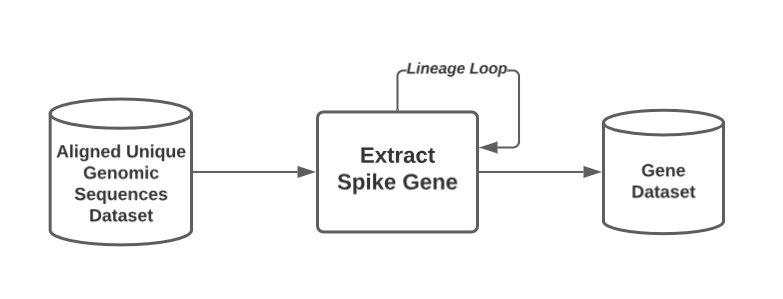
\includegraphics[scale=0.45]{figuras/pipelines/extracao_gene_spike.png}
          \fonte{O Autor}~\label{fig:extracaoSpike}
        \end{figure}
  \item \textbf{Filtragem de Sequências Genicas Duplicadas:} Uma das preocupações na criação do dataset foi a presença de sequências duplicadas, que podem enviesar os resultados da análise. Portanto, as sequências genômicas duplicadas foram identificadas e removidas do conjunto de dados. Esse processo garantiu que cada sequência fosse única, evitando redundâncias.
        \begin{figure}[htb]
          \centering
          \caption{Pipeline de Filtragem de Sequências Genicas Duplicadas.}
          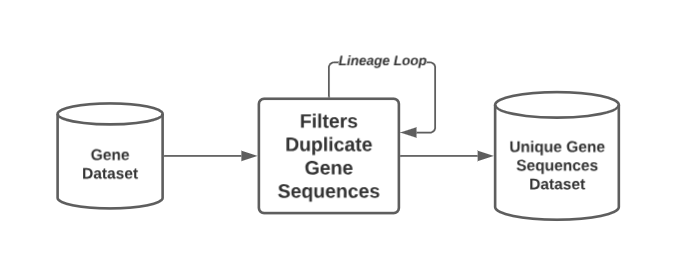
\includegraphics[scale=0.45]{figuras/pipelines/filtrando_spikes_duplicados.png}
          \fonte{O Autor}~\label{fig:spikeDuplicados}
        \end{figure}
  \item \textbf{Filtragem de Sequências de Má Qualidade:} Para garantir a qualidade do dataset, as sequências genômicas que continham características indesejáveis foram filtradas. Isso incluiu a remoção de sequências que continham mais de 30 bases nitrogenadas (N) consecutivas e aquelas que não correspondiam ao tamanho esperado das sequências de referência do gene spike como visto na imagem~\ref{fig:spikesRuins}. Essa filtragem ajudou a garantir que as sequências incluídas no dataset fossem de alta qualidade e relevantes para a análise subsequente.
        % FAZER: Corrigir parte que fala dos Ns
        \begin{figure}[htb]
          \centering
          \caption{Pipeline de Filtragem de Sequências Genicas de Má Qualidade.}
          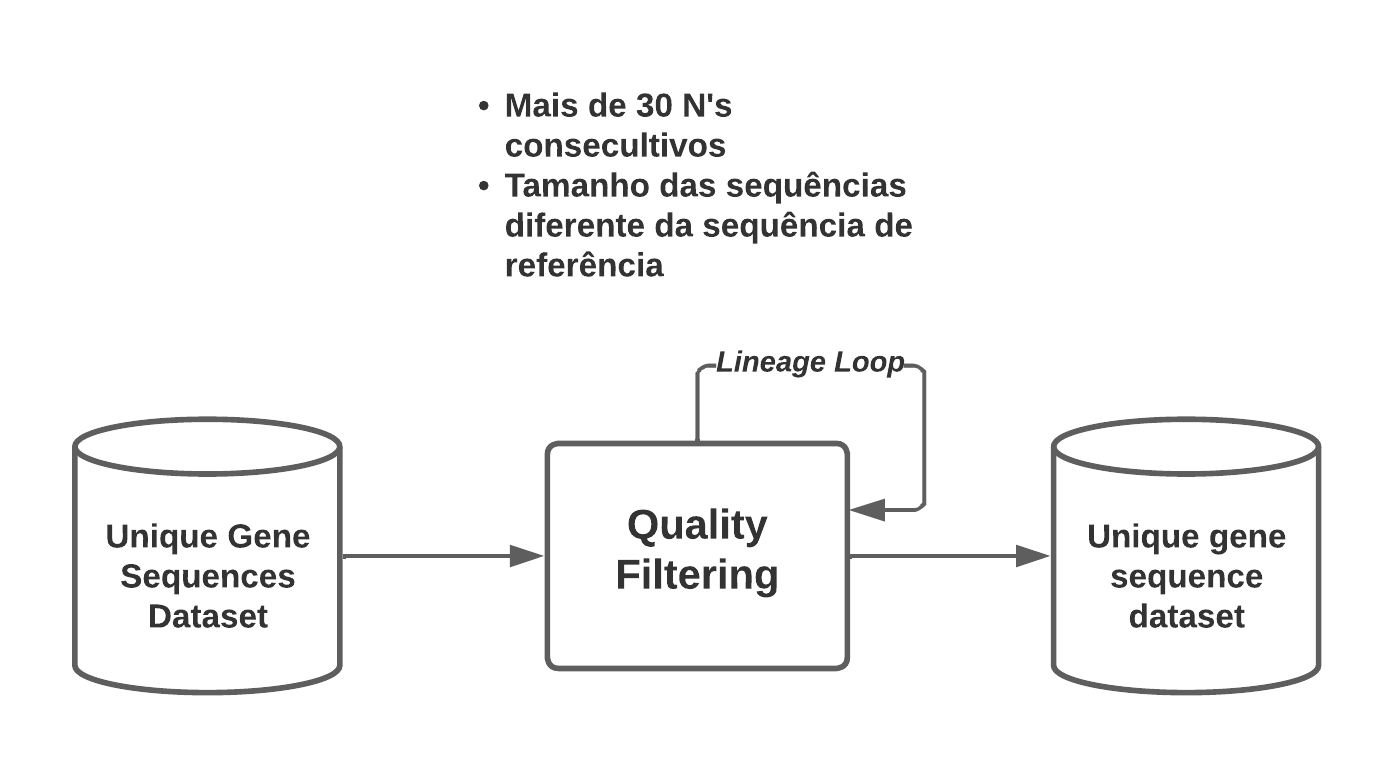
\includegraphics[scale=0.45]{figuras/pipelines/filtrando_spikes_ruins.png}
          \fonte{O Autor}~\label{fig:spikesRuins}
        \end{figure}
\end{enumerate}

Ao final do processo, foi gerado um \textit{dataset} de alta qualidade, contendo sequências gênicas únicas para as variantes alpha, beta, delta, gamma e omicron. Esse dataset será a base para a análise de genes virais com base no uso de códons e a aplicação de técnicas de classificação não supervisionada.

A partir deste dataset, foi elaborado 2 (dois) arquivos, conforme a figura~\ref{fig:inputAgua} apresenta, que serviria de entrada, tanto para o modelo desenvolvido como para a geração de árvores filogenéticas utilizando o modelo convencional, a fim de se realizar análises futuras. Um arquivo compreendia a mescla de sequências genicas de cada uma das linhagem, e um arquivo de anotações que serviria como base no treinamento, contendo o cabeçalho da sequência, na mesma ordem em que estava no arquivo mesclado, juntamente com a linhagem da sequência.

\begin{figure}[htb]
  \centering
  \caption{Arquivos de Entrada do AGUA.}
  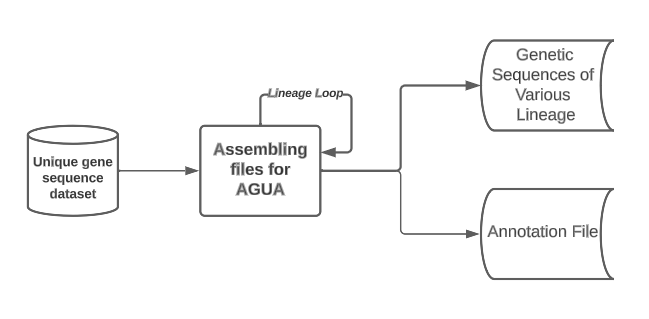
\includegraphics[scale=0.45]{figuras/pipelines/input_AGUA.png}
  \fonte{O Autor}~\label{fig:inputAgua}
\end{figure}

\subsection{AGUA}
O modelo proposto foi nomeado como \gls{agua}. A seguir o mesmo será apresentado, desde a sua concepção, implementação e testes.

% FAZER
% Escrever uma descrição melhor do desenvolvimento do modelo
\begin{itemize}
  \item Levantamento dos requisitos.
  \item Definir a arquitetura e a abordagem do modelo de classificação baseado em códons.
  \item Implementar o modelo utilizando uma biblioteca ou framework adequado.
  \item Desenvolver algoritmo para traduzir as sequências de \gls{dna} em sequências de códons.
  \item Realizar treinamento do modelo utilizando os dados preparados.
  \item Avaliar o desempenho do modelo utilizando métricas apropriadas.
        % \item \item Avaliar o desempenho do modelo utilizando métricas apropriadas, como acurácia, precisão e recall.
  \item Identificar possíveis problemas e realizar ajustes no modelo.
        % \item Identificar possíveis problemas de overfitting ou underfitting e realizar ajustes no modelo, como ajuste de hiperparâmetros ou utilização de técnicas de regularização.
\end{itemize}

\subsection{Análise comparativa entre o método proposto (AGUA) e outro método existente}

Nesta seção, apresentamos uma análise comparativa detalhada entre o método proposto e um método tradicional amplamente utilizado. O objetivo é avaliar o desempenho e a eficácia do nosso método em relação a uma abordagem estabelecida. Para esse fim, realizamos a análise em um conjunto de dados comum, utilizando o mesmo conjunto de dados que foi empregado na construção do nosso modelo, apresentado na figura~\ref{tab:datasetGenomasTeste}. O método tradicional selecionado para comparação é o utilizando o \textit{software} IQ-TREE, que é um estimador de máxima verossimilhança de alta performance, frequentemente empregado na filogenia molecular.~\cite{iqtree2_minh_2020}

A escolha do IQ-TREE como método tradicional se baseia em sua prevalência na comunidade científica e sua eficácia comprovada em construir árvores filogenéticas a partir de dados de sequenciamento. A avaliação comparativa entre o método proposto e o IQ-TREE nos permitirá avaliar a capacidade do nosso modelo em produzir resultados relevantes e precisos em comparação com uma abordagem estabelecida.

% FAZER Pontos importantes na análise comparativa
Nesta análise comparativa, examinaremos aspectos críticos da construção de árvores filogenéticas, como a topologia das árvores resultantes, a robustez das ramificações, e a resolução de agrupamentos de espécies. Além disso, consideraremos aspectos de escalabilidade e eficiência computacional.

A abordagem metodológica consiste em utilizar o mesmo conjunto de dados que alimentou nosso modelo para a construção de árvores filogenéticas usando o IQ-TREE como apresentado na figura~\ref{fig:inputAguaIqtree}. Comparamos, então, as árvores filogenéticas obtidas por ambos os métodos, avaliando suas similaridades e diferenças. Essa análise comparativa nos permitirá determinar se o método proposto representa uma melhoria significativa em relação à abordagem tradicional, contribuindo assim para o avanço no campo da filogenia molecular.

\begin{figure}[htb]
  \centering
  \caption{Arquivos de entrada do AGUA e do IQ-TREE.}
  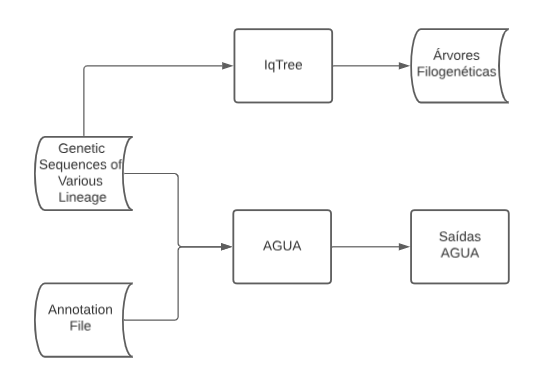
\includegraphics[scale=0.45]{figuras/pipelines/agua_iqtree.png}
  \fonte{O Autor}~\label{fig:inputAguaIqtree}
\end{figure}

% FAZER
% A seguir, descrevemos em detalhes a metodologia utilizada para realizar essa análise comparativa, bem como os resultados obtidos e suas implicações.
No contexto da análise comparativa realizada, o IQ-TREE foi aplicado ao mesmo conjunto de dados utilizado na construção do modelo proposto. Isso permitiu a geração de árvores filogenéticas com as linhagens corretamente separadas, como visto na figura~\ref{fig:arvoreIqtree}, que serviram como ponto de comparação para avaliar o desempenho do método proposto em relação a uma abordagem tradicional.

% FAZER
% Melhorar a figura
\begin{figure}[htb]
  \centering
  \caption{Árvore Filogenética Construída com o IQ-TREE.}
  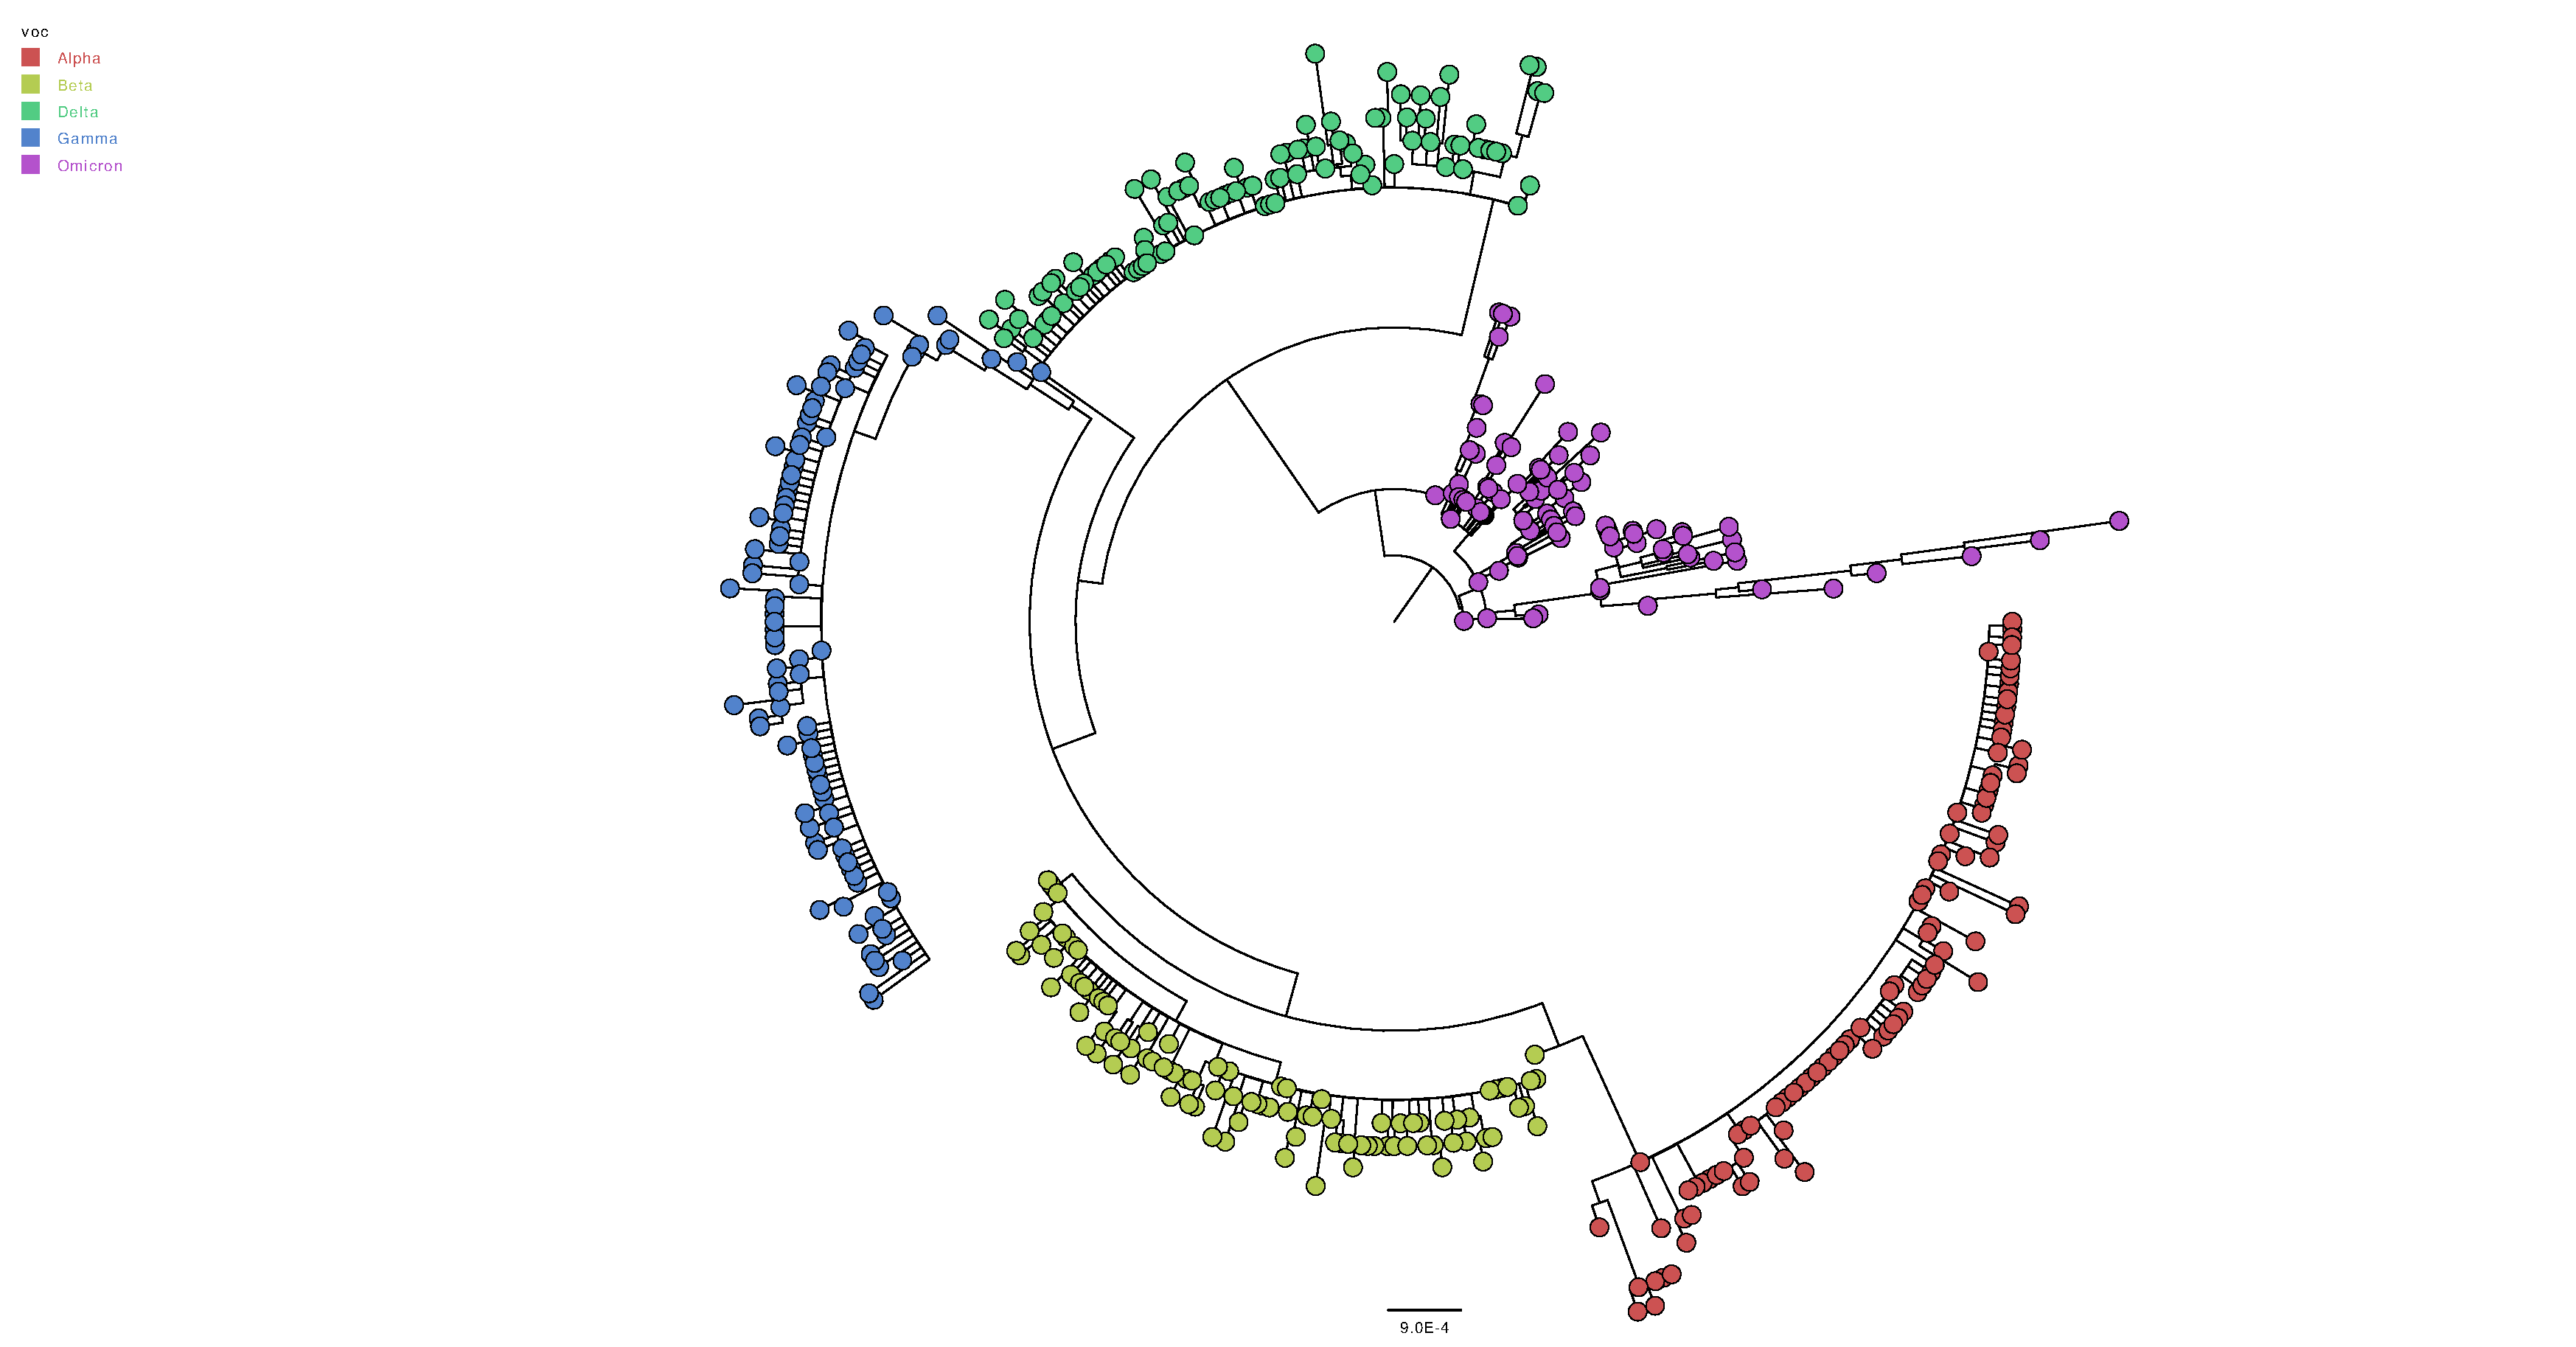
\includegraphics[scale=0.2]{figuras/filogenia_tradicional/sequencias_treinamento.fasta.treefile.pdf}
  \fonte{O Autor}~\label{fig:arvoreIqtree}
\end{figure}

% \begin{itemize}
%   \item Comparação dos métodos de agrupamento adotados, avaliando sua eficácia na formação de clusters e na identificação de padrões ou similaridades nas sequências.
%   \item Avaliação do custo computacional (tempo de execução e recursos requeridos) para a classificação das sequências em cada método.
%   \item Comparação da eficiência computacional entre os métodos, considerando a escalabilidade e o desempenho em grandes volumes de dados.
% \end{itemize}

% \section{Resultados Obtidos}